
\begin{concept}[15cm]
\textit{Mỗi chương trình bất kỳ đều cần một thiết kế tốt để giúp cho việc xây dựng dễ dàng và quy chuẩn hơn. Mục này sẽ trình bày cách mà bộ xử lý Windows API đã được hiện thực để tương tai sau này có thể dễ dàng sửa chữa, bảo trì và bổ sung thêm vào kiến trúc đó. Để hiểu rõ cấu chương trình mô phỏng câu lệnh assembly, sơ đồ class trình bày trong chương này thể hiện được mối quan hệ giữa các class, cấu trúc của chương trình BE-PUM được phát triển dựa trên dự án JakStab, giới thiệu các class quan trọng của chương trình BE-PUM.}
\end{concept}

\newpage
\section{Các câu lệnh hợp ngữ}
	\subsection{Sơ đồ chương trình BE-PUM}
		BE-PUM được xây dựng chủ yếu trên mã nguồn của JakStab do đó hình ~\ref{fig:SoDoClass} thể hiện phần BE-PUM đang được phát triền. \\

		Sơ đồ thể hiện mối liên hệ giữa các class với nhau. Trong sơ đồ không thể hiện các biến của class, các hàm của class, mục đích của sơ đồ thể hiện mối liên kết giữa các class với nhau. Class \textit{Program} là một class được phát triển từ dự án JakStab, BE-PUM kế thừa và phát triền lên. Class chính của BE-PUM là class \textit{Main}, nơi gọi chương trình cần phân tích. Class \textit{Main} sẽ gọi class \textit{OTFModelGeneration} để tạo ra sơ đồ CFG(control flow graph: sơ đồ điều khiển) với mỗi đỉnh là một câu lệnh assembly được dịch từ mã nhị phân của chương trình cần phân tích. Mỗi câu lệnh assembly có các biến môi trường khác nhau. Class \textit{Environment} có nhiệm vụ thể hiện môi trường làm việc của từng câu lệnh. Biến môi trường có các thành phần khác nhau như \textit{Register, Flag, Stack, Memory}cũng được hiện thực bằng các class tương ứng.
		
		\begin{center}
			\begin{figure}[htp]
				\begin{center}
					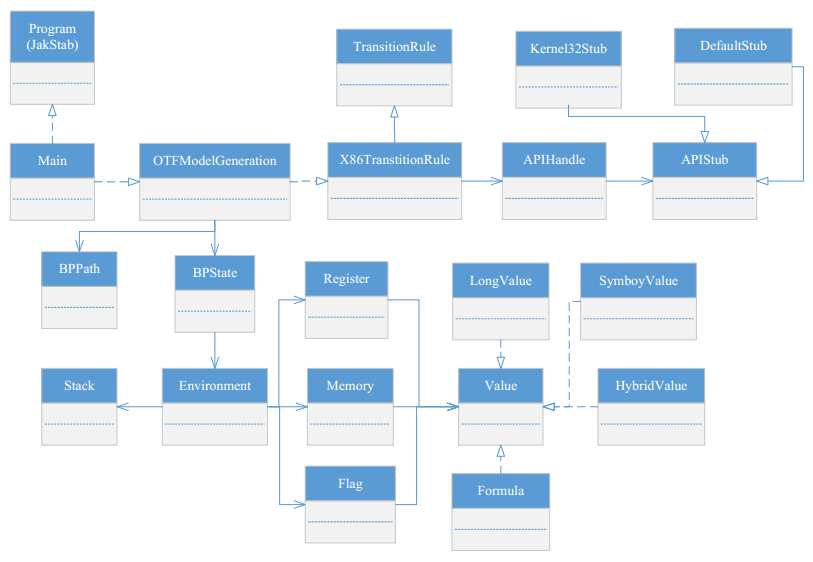
\includegraphics[scale=0.7]{SoDoClass.png}
				\end{center}
				\caption{Sơ đồ class chương trình BE-PUM}	
					\label{fig:SoDoClass}		
			\end{figure}
		\end{center}					
		
		Class  \textit{X86TransitionRule} có nhiệm vụ hiện thực mô phỏng các câu lệnh assembly. Để hiện thực mô phỏng các câu lệnh khác nhau, class \textit{X86TranstitionRule} được hỗ trợ thêm các class khác sẽ được trình bày trong phần "phân tích class mô phỏng câu lệnh Assembly". Class\textit{X86TranstitionRule} cũng đảm nhiệm việc tiến hành phân tích từng câu lệnh assembly, trong quá trình phân tích sẽ  co API (Microsoft Windows application programming interface) tham gia, vấn đề về API sẽ được đề cập đến phần "Window API".
		
		\newpage
	\subsection{Phân tích class mô phỏng câu lệnh Assembly}
	Hình ~\ref{fig:SoDoClassAss}	mô tả lược đồ lớp (class)  chính dùng đề mô phỏng câu lệnh assembly. Class quan trong \textit{X86TransitionRule} và\textit{Simulation Assembly} dùng để mô phỏng thao tác thực hiện của các câu lệnh assembly. Ngoài ra còn có class Environment mô phỏng các biến sẽ bị thay đổi khi câu lệnh assembly được thực thi. Các class \textit{FPUStatusWord, FPURegister, FPUControlWord} mô phỏng lại các biến môi trường mà các câu lệnh assembly xử lý FPU (Floatting-Point Unit) sử dụng. Class \textit{Register, Flag, Stack, Memory} mô phỏng lại các câu lệnh assembly thao tác trên số nguyên.\\
	
	Trong phần này sẽ phân tích môi trường cần để câu lệnh assembly xử lý số nguyên thực hiện và môi trường FPU xử lý số thực. Câu lệnh xử lý số nguyên và số thực tuy cùng mục đích thực hiện nhưng khi thao tác và thực hiện câu lệnh, các biến môi trường được sử dụng khác nhau. Nên việc thao tác, phân tách các biến môi trường sao cho phù hợp với hai nhóm xử lý số nguyên.	
		\begin{center}
			\begin{figure}[htp]
				\begin{center}
					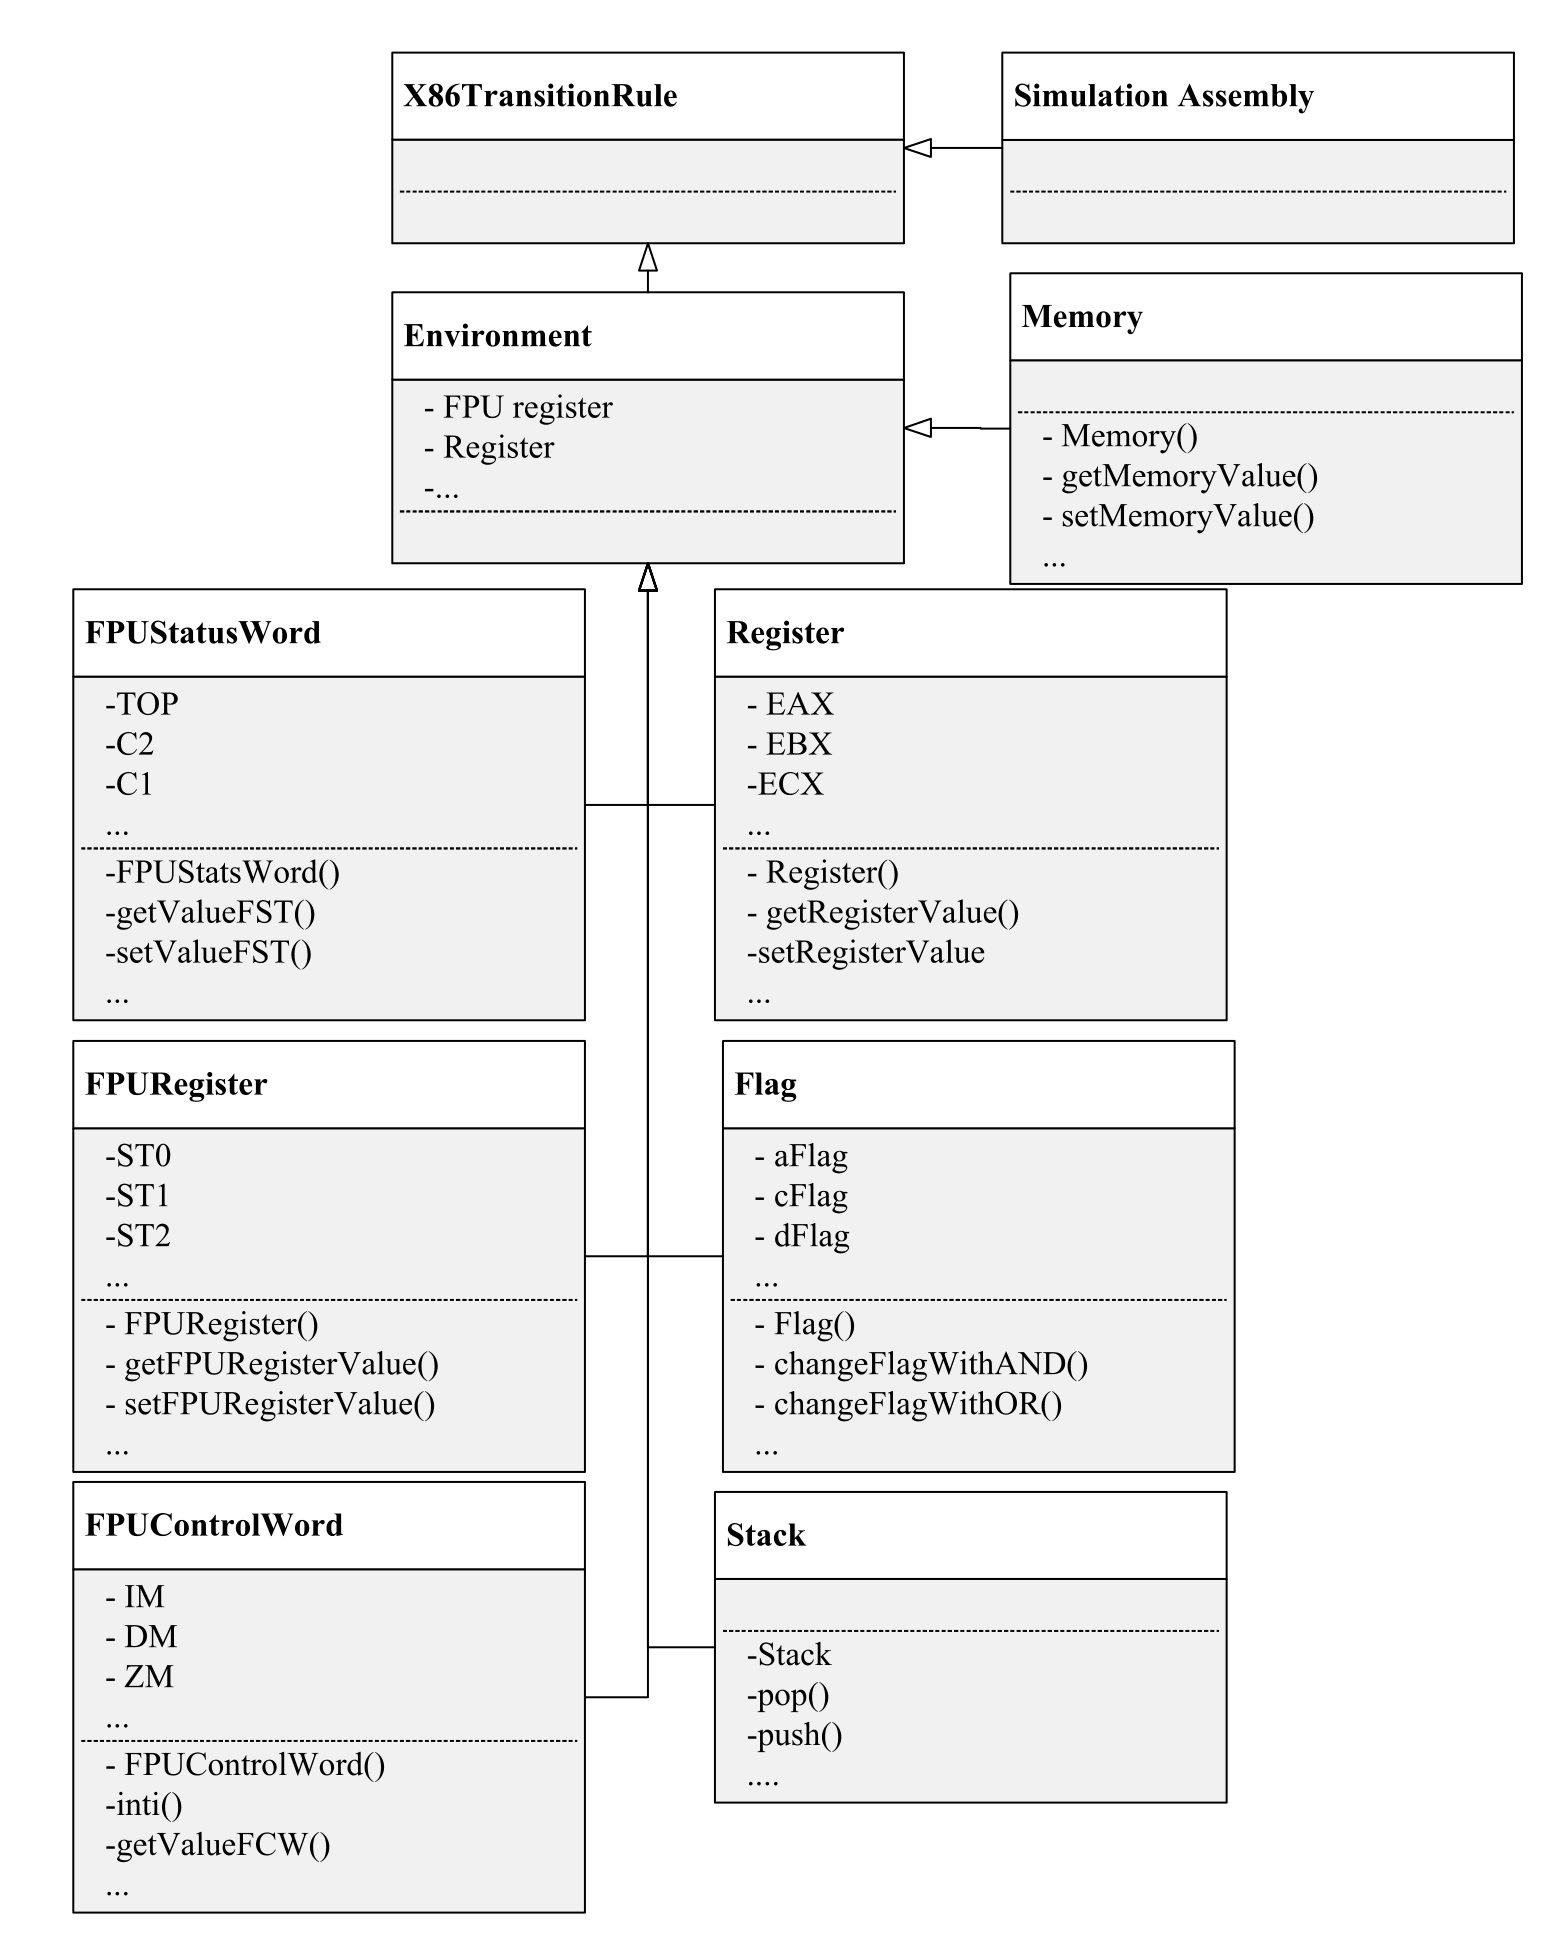
\includegraphics[scale=0.4]{UMLAss.png}
				\end{center}
				\caption{Sơ đồ class mô phỏng câu lệnh Assembly}	
					\label{fig:SoDoClassAss}		
			\end{figure}
		\end{center}			
		
		\newpage
		Để thể hiện các biến môi trường các class Register, Flag, Stack, FPUStatusWord, FPURegister, FPUControlWord,  Be-Pum xây dựng các class Environment để hỗ trợ trong việc truy xuất, thao tác.	
	
		\begin{center}
			\begin{figure}[htp]
				\begin{center}
					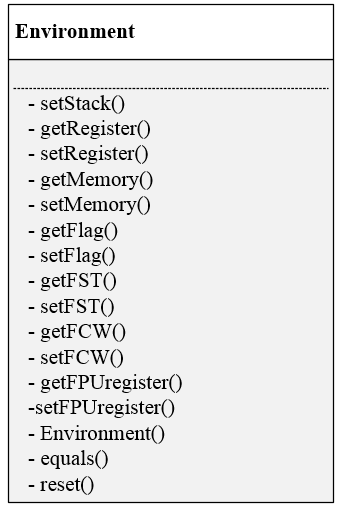
\includegraphics[scale=0.75]{ClassEnv.png}
				\end{center}
				\caption{Class Environment}	
					\label{fig:ClassEnv}		
			\end{figure}
		\end{center}					
		
		Class Environmet có nhiệm vụ liên kết các class Stack, Register, Memory, Flag, FPUStatusWord, FPURegister, FPUControlWord, để thao tác truy xuất trực tiếp lên các biến môi trường này. Class Enviroment hiện thực các hàm để hỗ trợ thao tác truy xuất thuận tiện hơn. Ngoài ra, hiện thực hàm equals() để so sánh biến môi trường của câu lệnh assembly này với biến môi trường của câu lệnh assembly khác. Từ đó hỗ trợ trong việc đánh giá, phân tích câu lệnh assembly.
		
	\newpage
	Class Simulation Assebmbly là một class abstract dùng để gọi các class với tên câu lệnh assembly tương ứng	
	\begin{center}
			\begin{figure}[htp]
				\begin{center}
					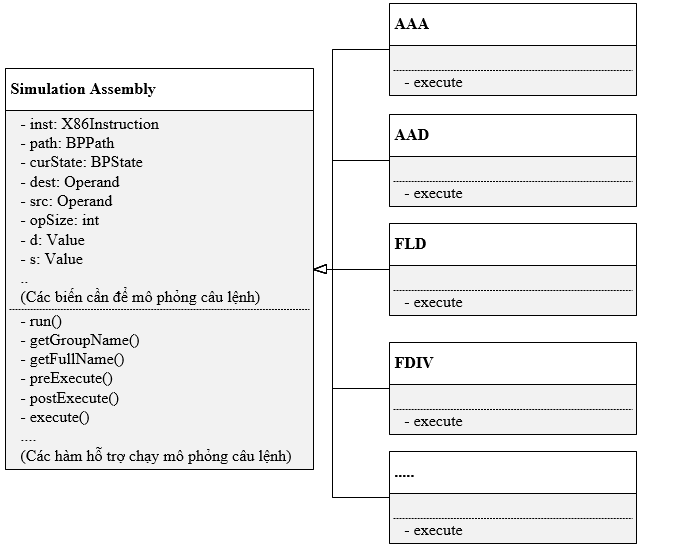
\includegraphics[scale=1.0]{ClassSimulation.png}
				\end{center}
				\caption{Class}	
					\label{fig:}		
			\end{figure}
		\end{center}				
		
		Class Simulation Assembly có nhiệm vụ hash tìm câu lệnh tương ứng với class để thực thi. Hàm execute() dùng để gọi lệnh thực thi tương ứng với câu lệnh đầu vào. Ngoài ra còn có các hàm getGroupName() hỗ trợ trong quá trình tìm kiếm được tối ưu. Hàm getFullName() hỗ trợ tìm kiếm với tên câu lệnh đầy đủ, không bị thiếu ký tự trong quá trình tìm kiếm class tương ứng. Ngoài ra có các biến dest, src lần lượt là toán hạng tương ứng với từng câu lệnh assembly được thực thi. 
		
		\newpage
	\subsection*{Môi trường xử lý số nguyên}
	Class Environmet liên kết với class Stack, hình~\ref{fig:ClassStack} thể hiện class Stack.
		\begin{center}
			\begin{figure}[htp]
				\begin{center}
					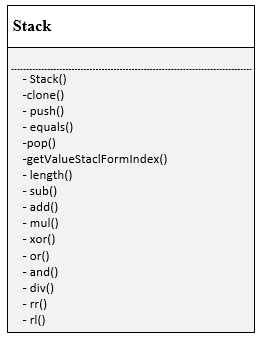
\includegraphics[scale=1.0]{ClassStack.png}
				\end{center}
				\caption{Class Stack}	
					\label{fig:ClassStack}		
			\end{figure}
		\end{center}		
	
	Class Stack gồm các hàm hỗ trợ thao tác trên stack của chương trinh. Hàm push() và pop() là hai hàm quan trọng có nhiệm vụ thao tác cơ bản trên stack là đưa vào ngăn xếp và lấy ngăn xếp ra. Ngoài ra còn có các hàm length() thể hiện kích thước stack, equals() để so sánh hai stack với nhau, việc này hỗ trợ rất nhiều trong qua trình phân tích hay so trùng được sử dụng trong các kỹ thuật phân tích virus. Ngoài ra còn có các hàm để hỗ trợ thao tác toán học như add() để cộng thêm một số, sub() để nhân với một số,…
			
		\newpage
		Class Register được hiện thực như các thanh ghi Register trong hợp ngữ assembly. Hình~\ref{fig:ClassRegister} thể hiện class Register:
		\begin{center}
			\begin{figure}[htp]
				\begin{center}
					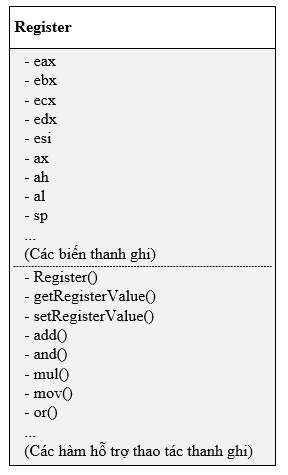
\includegraphics[scale=1.0]{ClassRegister.png}
				\end{center}
				\caption{Class Register}	
					\label{fig:ClassRegister}		
			\end{figure}
		\end{center}		
			
	Class Register gồm các biến được thể hiện là các thanh ghi Register được sử dụng trong hợp ngữ assembly. Các biến này sẽ lưu giá trị của thanh ghi trong quá trình thực thi chương trình cần phân tích. Mỗi giá trị của biến có thể bị thay đổi khi thực hiện phân tích từng câu lệnh assembly của chương trình cần phân tích. Class Resgister xây dựng các hàm hỗ trợ thao tác trên thanh ghi như getRegiterValue() có nhiệm vụ lấy giá trị của thanh ghi nào đó, setRegisterValue() có nhiệm vụ gán lại giá trị của một thanh ghi. Ngoài ra, class Register còn hiện thực một số hàm hỗ trợ thao tác toán học trên thanh ghi như: add() có nhiệm vụ cộng thêm một giá trị nào đó vào thanh ghi, and() có nhiệm vụ như thực hiện phép and (đại số Boole),.. những hàm này giúp hỗ trợ nhanh trong việc hiện thực câu lệnh sau này.
	
		\newpage
	Class Memory được hiện thực như là các thao tác trên một bộ nhớ được sử dụng trong hợp ngữ assembly. Hình~\ref{fig:ClassMemory} thể hiện class Memory: 
	
		\begin{center}
			\begin{figure}[htp]
				\begin{center}
					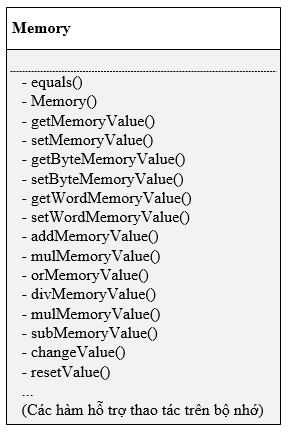
\includegraphics[scale=1.0]{ClassMemory.png}
				\end{center}
				\caption{Class Memory}	
					\label{fig:ClassMemory}		
			\end{figure}
		\end{center}		
	
	Class Memory gồm các hàm được hiện thực để hỗ trợ trong việc thao tác với địa chỉ bộ nhớ. Mỗi hàm được hiện thực có nhiệm vụ khác nhau nhưng cùng một mục đích là phân tích câu lệnh assembly như hàm equals() dùng để so sánh bộ nhớ, getMemoryValue() dùng để lấy giá trị của địa chỉ bộ nhớ đó, setMemoryValue() dùng để gán lại giá trị của bộ nhớ, getByteMemoryValue() dùng để lấy giá trị Byte của địa chỉ bộ nhớ, ngoài ra còn có các hàm hỗ trợ thao tác toán học được sử dụng trên bộ nhớ như hàm addMemoryValue() dùng để cộng thêm một số vào giá trị bộ nhớ, mulMemoryValue() dùng để nhân thêm một số vào giá trị bộ nhớ, changeValue() với địa chỉ xác định dùng để thay đổi giá trị của địa chỉ bộ nhớ đó, việc thay đổi giá trị tại địa chỉ bộ nhớ giúp hỗ trợ trong quá trình phân tích, đọc hiểu mã assembly.
	
	\newpage
	Class Flag được hiện thực như các Flag trong hợp ngữ assembly. Hình~\ref{fig:ClassFlag} thể hiện class Flag của chương trình BE-PUM:	
		\begin{center}
			\begin{figure}[htp]
				\begin{center}
					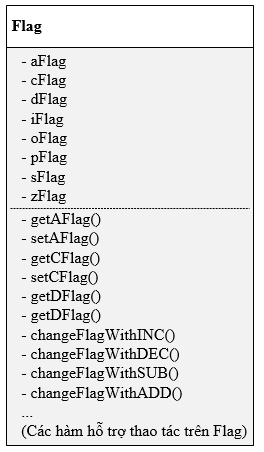
\includegraphics[scale=1.0]{ClassFlag.png}
				\end{center}
				\caption{Class Flag}	
					\label{fig:ClassFlag}		
			\end{figure}
		\end{center}			
	
Class Flag gồm các biến được phỏng theo các biến Flag được sử dụng trong hợp ngữ assembly, mỗi tên biến tương với mỗi giá trị Flag trong quá trình phân tích. Các giá trị của Flag sẽ thay đổi theo từng câu lệnh assembly, dựa vào xự thay đổi này để hỗ trợ trong quá trình phân tích chương trình. Ngoài ra, class Flag còn hiện thực thêm một số hàm để hỗ trợ trong quá trình phân tích như getAFlag() để lấy giá trị của aFlag, setAFlag() để thay đổi giá trị của aFlag, tương tự như vậy đối với các biến đã được mô phỏng. Thêm vào đó là các hàm thay đổi Flag theo các câu lệnh hỗ trợ toán học như hàm changeFlagWithINC() có nhiệm vụ thay đổi các giá trị của Flag tương ứng khi thực hiện câu lệnh INC (tăng giá trị), changeFlagWithSUB() thay đổi Flag khi thực hiện phép toán công (SUB),… Tương tự như vậy, class tiếp tục xây dựng các hàm hỗ trợ thay đổi nhanh khi thực hiện các phép toán.


	\newpage
	Class X86TranstitionRule là class đặc biệt quan trọng, là nơi xử lý các câu lệnh assembly, class X86TranstitionRule được hỗ trợ bởi nhiểu class con khác để thực hiện việc phân tích mã assembly. Hình~\ref{fig:X86TransitionRule	} biểu diễn class X86TranstitionRule:
	\begin{center}
			\begin{figure}[htp]
				\begin{center}
					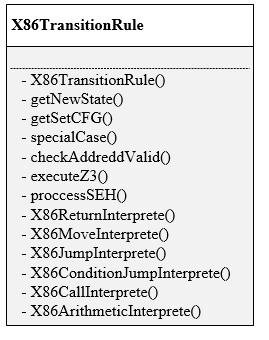
\includegraphics[scale=1.0]{ClassTransitionRule.png}
				\end{center}
				\caption{Class X86TransitionRule	}	
					\label{fig:X86TransitionRule	}		
			\end{figure}
		\end{center}			
		
	Class X86TransitionRule được hiện thực các hàm để hỗ trợ trong quá trình phân tích chương trình assembly. Mỗi đỉnh trong đồ thị phân tích là một câu lệnh, mỗi câu lệnh có nhiệm vụ, chức năng khác nhau. Do đó, cần phần nhóm các câu lệnh để hiện thực. Trong class X86TransitionRule, các hàm được chia theo nhóm câu lệnh như X86IntrustionInterprete() hiện thực các câu lệnh cơ bản thường dùng như STD (gán giá trị dFlag = 1) cmovcc (các điều kiện gán)… X86RetrunInterprete() hiện thực các câu lệnh trả kết quả về như RET (kết quả trả về khi kết thúc một hàm), X86MoveInterprete() hiện thực các câu liên quan đến gán giá trị như MOV, MOVZ,… tương tự như vậy các nhóm câu lệnh nhảy, biểu thức toán học, các câu lệnh gọi hàm được hiện thực. Ngoài ra còn có các hàm hỗ trợ trong việc phân tích và tính toán như hàm executeZ3() có nhiệm vụ gọi thư viện Z3 để tính toán. Đây làm class rất quan trọng vì class này đảm nhận nhiệm vụ phân tích chương trinh assmebly từ đó đưa ra kết quả.
	
	\newpage	
	\subsection*{Môi trường xử lý số thực}
	Class FPUControlWord mô phỏng thanh ghi Control Word FPU. Hình ~\ref{fig:FPUControlWord} biểu diễn các biến và hàm quan trọng trong để mô phỏng thanh ghi điều kiển FPU.	
		\begin{center}
			\begin{figure}[htp]
				\begin{center}
					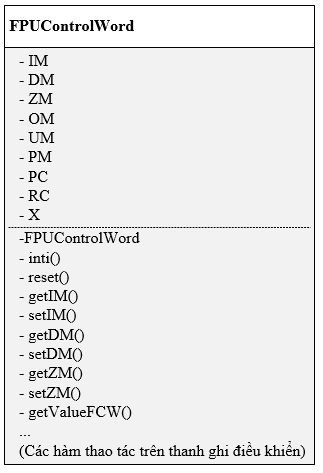
\includegraphics[scale=1.0]{ClassFCW.png}
				\end{center}
				\caption{Class FPUControlWord	}	
					\label{fig:FPUControlWord}		
			\end{figure}
		\end{center}		
			
		Class FPUControlWord chứa các biến IM, DM, ZM, ... tương ứng với các bit cờ trong thanh ghi điều khiển FPU. Mỗi biến biểu diễn một bit trong thanh ghi. Hàm getValueFCW() trả giá trị hex, việc trả giá trị hex giúp so sanh, kiểm tra kết quả nhanh hơn. Ngoài ra còn các hàm hỗ trợ truy xuất, thiết lập các biến IM, DM, ZM... giúp thuận tiện trong quá trình hiện thực các câu lệnh, thay đổi giá trị trong thanh ghi điều khiển FPU. Hàm inti() thiết lập các thông số ban đầu của thanh ghi điều khiển FPU. 
		
		\newpage
		Class FPUStatusWord mô phỏng thanh ghi Status Word FPU. Hình ~\ref{fig:FPUStatusWord} biểu diễn các biến và hàm quan trọng trong để mô phỏng thanh ghi trạng thái FPU.	
	\begin{center}
			\begin{figure}[htp]
				\begin{center}
					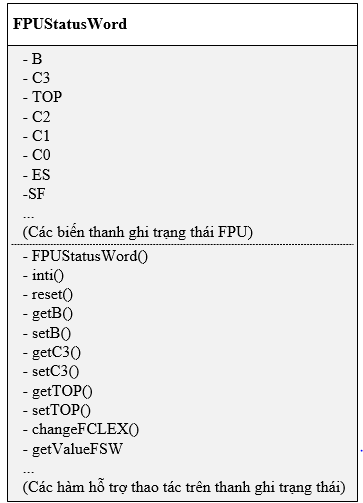
\includegraphics[scale=1.0]{ClassFSW.png}
				\end{center}
				\caption{Class FPUStatusWord	}	
					\label{fig:FPUStatusWord}		
			\end{figure}
		\end{center}			
		
		Class FPUStatusWord mô phỏng các bit được sử dụng trong thanh ghi trạng thái FPU tương ứng với các biên B, C3, TOP, C2, .... Mỗi biến biểu diễn một bit trong thanh ghi, riêng biến TOP tương ứng với giá trị đỉnh của stack được biểu diễn bằng số nguyên. Class FPUStatusWord có các hàm hỗ trợ trong việc truy xuất và thiết lập các biển getB(), setB(),... Hàm getValueFSW() trả về giá trị hex, việc trả giá trị hex giúp kiểm tra và so sánh kết quả của từng câu lệnh assembly sau khi thực hiện xong. Hàm inti() thiết lập các thông số ban đầu cho thanh ghi trạng thái FPU.
		
		\newpage
		Class FPURegister mô phỏng stack thanh ghi dữ liệu FPU. Hình~\ref{fig:FPUreg} biểu diễn các biến và hàm quan trọng trong để mô phỏng stack thanh ghi dữ liệu FPU.	
	\begin{center}
			\begin{figure}[htp]
				\begin{center}
					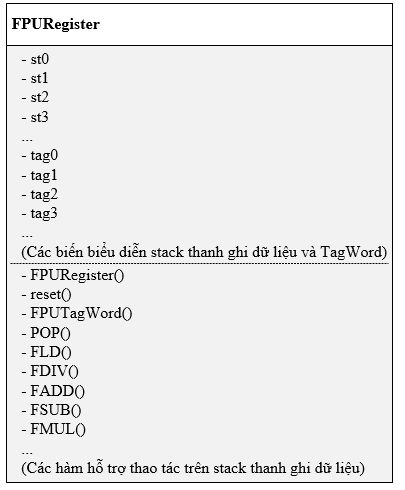
\includegraphics[scale=1.0]{ClassFPUReg.png}
				\end{center}
				\caption{Class stack thanh ghi dữ liệu FPU}	
					\label{fig:FPUreg}		
			\end{figure}
		\end{center}			
	
		Class FPURegister có các biến ST0, ST1, ST2,.. lần lượt tương ứng với các stack thanh ghi dữ liệu được dùng để thao tác trong xử lý dấu chấm động. Các biến tag0, tag1, tag2,... tương ứng với các biến trong thanh ghi Tag Word được mô phỏng lại. Các biến tag dùng để chỉ trạng thái thanh ghi dữ liệu đang lưu trữ số có hợp lệ hay không. Class có các hàm hỗ trợ trong việc thao tác trên stack thanh ghi dữ liệu FPU. Hàm pop() lấy thanh ghi đỉnh của stack ra ngoài. Hàm FLD() dùng để nạp giá trị vào stack thanh ghi dữ liệu. Các hàm FDIV(), FADD(), FSUB(), FMUL() hỗ trợ trong việc thao tác toán học trên stack thanh ghi dữ liệu FPU.
		
		\newpage
		\subsection{Quy trình thực hiện}		
		Với những biến môi trường được mô phỏng lại để hiện thực và kiểm tra kết quả chính xác của từng câu lệnh. Mỗi câu lệnh có những thao tác riêng trên những biến môi trường khác nhau vì vậy để đảm bảo tính chính xác khi hiện thực, trong quá trình hiện thực cần phải xây dựng các test-case để kiểm tra. Hình ~\ref{fig:HienThucAss} thể hiện quy trình hiện thực một câu lệnh assembly.
		\begin{center}
			\begin{figure}[htp]
				\begin{center}
					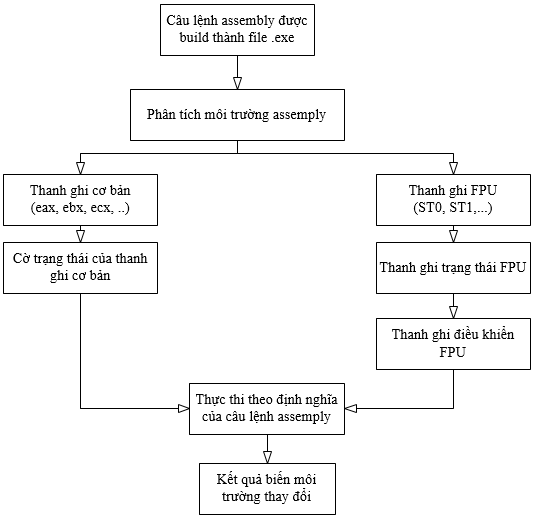
\includegraphics[scale=1.0]{HienThucAss.png}
				\end{center}
				\caption{Quy trình hiện thực một câu lệnh assembly}	
					\label{fig:HienThucAss}		
			\end{figure}
		\end{center}		
				
		Mỗi câu lệnh được xây dựng và build thành một file thực thưc có đuôi file là .exe. Mỗi câu lệnh thao tác trên các môi trường khác nhau có thể là môi trường số nguyên hoặc môi trường số thực. Sau khi phân loại để xác định môi trường thay đổi của câu lệnh assembly cần, bước tiếp theo xây dựng mô phỏng quá trình thực thi của câu lệnh đó. Mỗi câu lệnh có thao tác khác nhau trên môi trường thực hiện do đó kết quả cũng khác nhau. Kết quả thu được là biến môi trường sẽ bị thay đổi.\\
		
		Để kiểm tra kết quả đó đúng hay sai cần sử dụng thêm công cụ Ollydbg \footnote{Xem trong phần Phụ lục 2}. Hình ~\ref{fig:SoSanhAss} thể hiện quy trình kiểm tra kết quả của một câu lệnh assmebly.
			\begin{center}
			\begin{figure}[htp]
				\begin{center}
					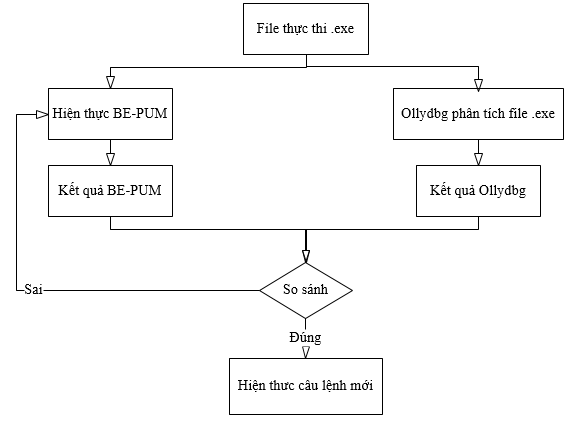
\includegraphics[scale=1.0]{SoSanhAss.png}
				\end{center}
				\caption{So sánh kết quả với Ollydbg}	
					\label{fig:SoSanhAss}		
			\end{figure}
		\end{center}			
		
		Khi một file thực thi .exe tương ứng với một câu lệnh assmebly là đầu vào cho công cụ Ollydbg. Kết quả Ollydbg cho biết sự thay đổi môi trường mà câu lệnh assembly đó thực hiện. Giả sử kết quả Ollydbg hoàn toàn chính xác và lấy kết quả đó làm chuẩn cho kết quả mà BE-PUM mô phỏng lại. Nếu kết quả BE-PUM trả về sai so với kết quả Ollđbg, sẽ hiện thực lại câu lệnh đó trong BE-BUM. Ngược lại, nếu đúng thì thực hiện tiếp các câu lệnh assembly khác
		
\newpage
\section{Windows API} \label{sec:wapi_design}

	\subsection{Các thành phần chính của bộ xử lý Windows API} \label{sec:main_classes}

	\begin{figure}[htp]
	\centering
		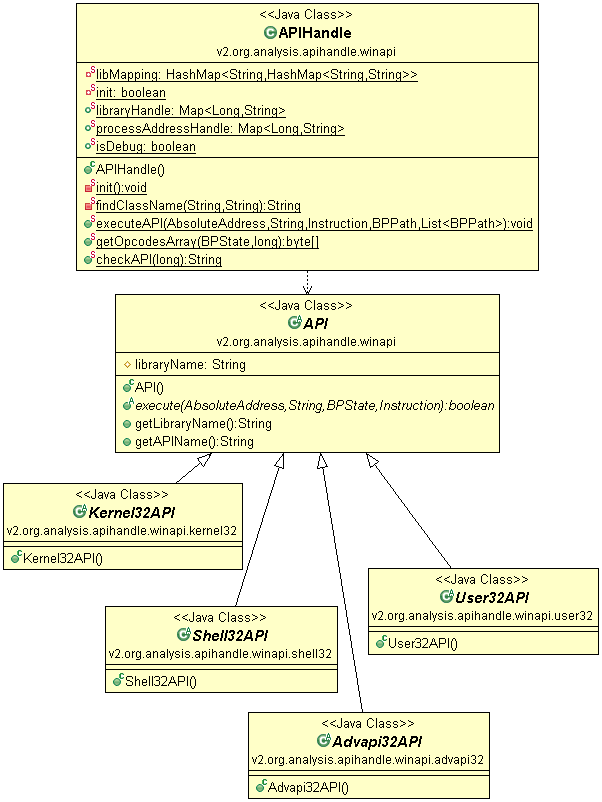
\includegraphics[scale=0.74]{wapi_1_main_classes.png}
		\caption{Kiến trúc chính của bộ xử lý Windows API dành cho BE-PUM}	
		\label{fig:wapi_1_main_classes}		
	\end{figure}

Hình \ref{fig:wapi_1_main_classes} mô tả lược đồ lớp (class) chính được xây dựng cho bộ xử lý Windows API. Trong đó có một class nắm giữ toàn bộ giao tiếp và làm việc giữa hệ thống BE-PUM và các xử lý chính cho từng API đó là class \textit{APIHandle}. Mỗi khi hệ thống BE-PUM cần xử lý một API bất kỳ nào đó, phương thức \textit{executeAPI} của \textit{APIHandle} sẽ được gọi để làm việc.\\

Kiến trúc chính của đề tài được xây dựng dựa trên dạng thức thiết kế adapter hay còn gọi là dạng thiết kế điều hợp. Với adapter là lớp trừu tượng – abstract class: lớp \textit{API}, mỗi bộ thư viện Windows API sẽ được trừu tượng hóa thành từng abstract class mà sẽ kế thừa từ lớp \textit{API} (ví dụ như các lớp \textit{Kernel32API}, \textit{User32API},…). Rồi sau đó, mỗi Windows API sẽ được trừu tượng hóa thành một class, được đặt tên trùng với tên của chính Windows API đó, kèm theo sẽ là việc kế thừa và hiện thực đúng abstract class của bộ thư viện mà Windows API thuộc về.\\

Hình \ref{fig:wapi_2_implemented_classes} ngay sau đây sẽ mô tả ngắn gọn cho việc hiện thực từng Windows API của bộ thư viện dịch vụ nền được chứa trong tập tin \textit{kernel32.dll}.

	\begin{figure}[htp]
	\centering
		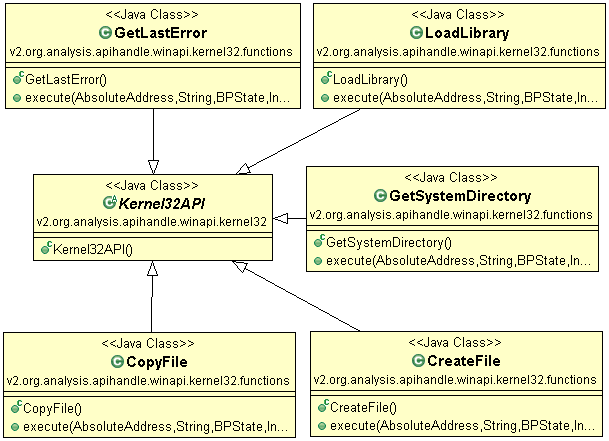
\includegraphics[scale=0.74]{wapi_2_implemented_classes}
		\caption{Mô hình hiện thực một số Windows API trong \textit{kernel32.dll}}	
		\label{fig:wapi_2_implemented_classes}		
	\end{figure}

	\newpage
	\subsection{Những khai báo ánh xạ của bộ xử lý Windows API} \label{sec:mapping}

Ngoài những thành phần chính nêu trên, bộ xử lý Windows API còn có những lớp khác để nắm thông tin ánh xạ giữa hai ngôn ngữ lập trình Java và C thông qua JNA.

	\begin{figure}[H]
	\centering
		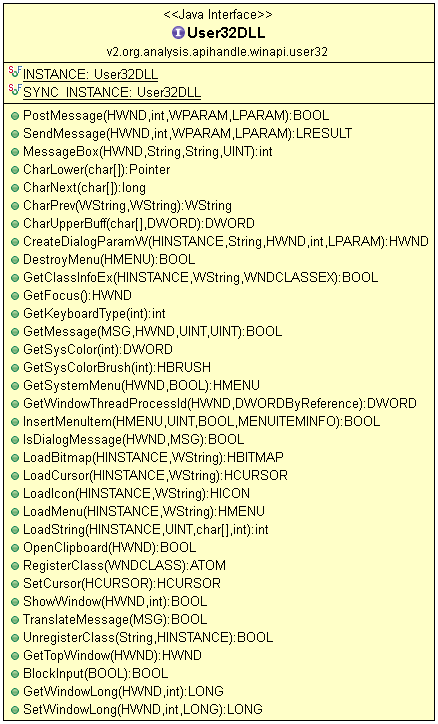
\includegraphics[scale=0.74]{wapi_3_function_map.png}
		\caption{Lớp chứa thông tin ánh xạ những Windows API trong \textit{user32.dll}}	
		\label{fig:wapi_3_function_map}		
	\end{figure}

Trong Hình \ref{fig:wapi_3_function_map} là một mô tả về ánh xạ tên hàm và kiểu dữ liệu đầu vào của bộ thư viện giao diện người dùng được chứa trong tập tin \textit{user32.dll}. Ngoài ra, bộ thư viện JNA có khai báo ánh xạ sẵn một số hàm Windows API cùng những kiểu dữ liệu chính mà Windows API thường dùng, nhờ đó mà những kiểu dữ liệu thông dụng như \textit{HWND, HINSTANCE, LPARAM, DWORD,…} không đòi hỏi lập trình viên phải khai báo và ánh xạ lại.\\

Nhưng không phải tất cả kiểu dữ liệu đề có sẵn, đặc biệt là những kiểu dữ liệu cấu trúc, cần có những trường hợp phải khai báo thêm để ánh xạ và phục vụ cho đề tài này.

	\begin{figure}[H]
	\centering
		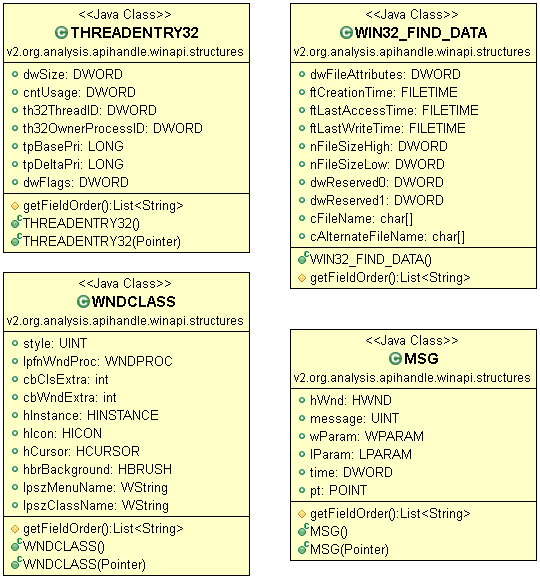
\includegraphics[scale=0.74]{wapi_4_structure}
		\caption{Một số dữ liệu kiểu cấu trúc được xây dựng thêm}	
		\label{fig:wapi_4_structure}		
	\end{figure}

Nội dung của Hình \ref{fig:wapi_4_structure} thể hiện khai báo thêm của một số dữ liệu kiểu cấu trúc dành cho đề tài này. Như đã nói ở Mục \ref{sec:structure}, việc xây dựng này đòi hỏi phải chính xác về kích thước và trình tự các biến được khai báo bên trong struct, để dữ liệu được nạp ra vào chính xác.

	\subsection{Kiến trúc xây dựng và làm việc}

Từ những thành phần đã trình bày ở Mục \ref{sec:main_classes} và Mục \ref{sec:mapping}, kiến trúc của bộ xử lý Windows API sẽ được tổ chức lại cho thống nhất và dễ dàng mở rộng về sau:

	\begin{figure}[H]
	\centering
		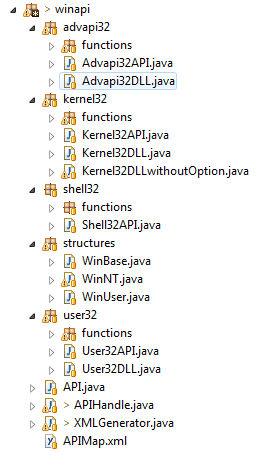
\includegraphics[scale=0.74]{wapi_5_tree}
		\caption{Cây cấu trúc mô tả những thành phần trong bộ xử lý Windows API}	
		\label{fig:wapi_5_tree}		
	\end{figure}

Gói ngoài cùng của bộ xử lý \textit{(winapi)} sẽ nắm:
\begin{itemize}
	\item Khai báo lớp trừu tượng \textit{API}: đặc tả phương thức thực thi dùng chung cho mọi Windows API;
	\item Lớp \textit{APIHandle}: giao tiếp chính giữa bộ xử lý Windows API và hệ thống BE-PUM;
	\item Những gói được đặt tên ứng với từng tên tập tin (không bao gồm phần mở rộng) mà bộ thư viện đó thuộc về. Mỗi gói đó sẽ chứa những thành phần như sau:
	
	\begin{itemize}
		\item Lớp khai báo trừu tượng cho từng Windows API của bộ thư viện đó (ví dụ như lớp \textit{Kernel32API}), trong đó sẽ nạp vào tên của bộ thư viện hiện tại;
		\item Lớp khai báo ánh xạ thư viện và tên hàm mà hiện bộ thư viện JNA chưa có sẵn (chỉ tồn tại trong trường hợp những Windows API mà đề tài hiện thực chưa có trong bộ thư viện JNA)
		\item Một gói được đặt tên \textit{functions}: dùng để chứa mọi lớp xử lý cho từng Windows API của bộ thư viện hiện tại (ví dụ như hiện tại gói bên ngoài là \textit{kernel32}, những hàm Windows API được xây dựng bên trong sẽ là: \textit{CreateFile, CopyFile, GetLastError…}).
	\end{itemize}
	\item Gói \textit{structures}: chứa những lớp khai báo ánh xạ dữ liệu kiểu cấu trúc mà bộ thư viện JNA chưa có sẵn.
	\item Lớp \textit{XMLGenerator}: có chức năng sinh ra tự động tập tin cấu trúc XML từ tổ chức như trên của bộ xử lý Windows API, mô tả ánh xạ giữa tên của hàm Windows API và tên đầy đủ của lớp sẽ đảm nhận việc xử lý hàm Windows API đó, kèm theo là nó thuộc tập tin thư viện nào. Ví dụ như sau:
\begin{boxedminipage}{12cm}
\begin{small}
\lstset{language=HTML}
\begin{lstlisting}
<APIMap>
	<DLL name="advapi32">
		<API funcName="cryptdecrypt" 
className="advapi32.functions.CryptDecrypt"/>
	</DLL>
	<DLL name="kernel32">
		<API funcName="closehandle" 
className="winapi.kernel32.functions.CloseHandle"/>
	</DLL>
</APIMap>
\end{lstlisting}
\end{small}
\end{boxedminipage}
	\item Tập tin \textit{APIMap.xml}: là nội dung do lớp \textit{XMLGenerator} sinh ra.
\end{itemize}

Nội dung của tập tin \textit{APIMap.xml} được sinh ra dùng để làm chỉ mục cho lớp trung gian \textit{APIHandle} biết được rằng: với thông tin đầu vào là tên của Windows API mà hệ thống BE-PUM yêu cầu, thì lớp nào sẽ xử lý được yêu cầu đó. Sau khi có được tên đầy đủ của lớp xử lý, \textit{APIHandle} sẽ khởi tạo lớp đó với kiểu đối tượng là \textit{API} (do tất cả lớp xử lý đều hiện thực trên lớp này), rồi sau đó gọi phương thức \textit{execute} để đối tượng này xử lý toàn bộ.

	\begin{figure}[H]
	\centering
		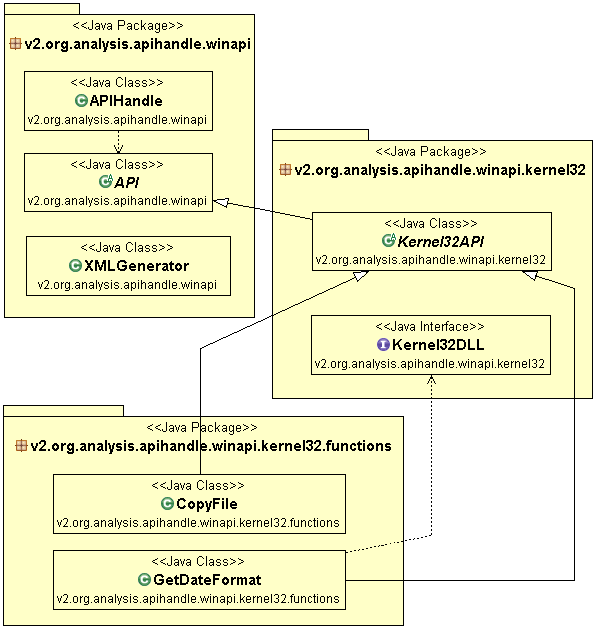
\includegraphics[scale=0.74]{wapi_6_inherited}
		\caption{Giản đồ thể hiện mối liên hệ giữa các thành phần}	
		\label{fig:wapi_6_inherited}		
	\end{figure}

\newpage
Với việc tổ chức theo cấu trúc này và sinh ra tập tin đánh chỉ mục thì sẽ có được những ưu điểm sau đây:

\begin{itemize}
	\item Dễ dàng quản lý mã nguồn: do Windows API có rất rất nhiều hàm, việc tạo ra mỗi lớp độc lập để xử lý cho từng hàm Windows API sẽ giúp cho mã nguồn được rõ ràng và độc lập cũng như việc sửa chữa sau này được tiện lợi;

	\item Dễ dàng bổ sung: nếu muốn hiện thực thêm một Windows API bất kỳ, ta chỉ việc tạo ra một lớp theo đúng quy định cấu trúc như trên, lớp XMLGenerator sẽ giúp sinh ra nội dung của tập tin APIMap.xml và chỉ đơn giản như vậy là đã tích hợp được một Windows API mới.
\end{itemize}

Nội dung của Hình \ref{fig:wapi_6_inherited} trình bày ví dụ về mối liên hệ mà cấu trúc vừa nêu. Khi hệ thống BE-PUM yêu cầu lớp APIHandle xử lý hàm CopyFile, nó sẽ dùng APIMap.xml để tìm được tên đầy đủ của lớp xử lý được hàm này. Tên ấy được dùng để khai báo khởi tạo động một đối tượng bất kỳ và sau đó ép kiểu về kiểu đối tượng API. Do lớp xử lý được hàm này được hiện thực dựa trên lớp trừu tượng API. Còn với trường hợp nếu là hàm GetDateFormat, thì trong lớp này còn có sử dụng lớp Kernel32DLL do bộ thư viện JNA chưa khai báo sẵn hàm này.

	\subsection{Quản lý môi trường tương tác vật lý}

Do một số Windows API có khả năng làm việc với hệ thống tập tin lưu trữ, dẫn đến khả năng làm ảnh hưởng xấu đến hệ thống do chúng ta đang tập trung vào việc phân tích những phần mềm độc hại cho máy vi tính. Vì vậy ta cần quản lý và ngăn chặn việc đó.\\

Để hiện thực việc đó, một lớp mang tên \textit{Storage} được viết ra để ánh xạ toàn bộ địa chỉ của hệ thống thật vào một vùng lưu trữ đã được quy định. Và rồi mỗi khi một Windows API nào có sử dụng đường dẫn để làm việc, thì cần phải kiểm tra rằng liệu Windows API đó có khả năng ảnh hưởng đến hệ thống hay không, nếu có ta cần ánh xạ sang vùng lưu trữ đã được quản lý để tránh những nguy hại.
